% Chapter 5

\chapter{Evaluation} % Main chapter title

\label{Chapter5}

\lhead{Chapter 5. \emph{Evaluation}} % This is for the header on each page - perhaps a shortened title

%----------------------------------------------------------------------------------------

% \emph{Beskriv hvordan du vurderer arbeidet ditt. Oppsummer evalueringsresultatene, og bruk dem til å vurdere ditt eget arbeid kritisk. Vær ærlig om eventuelle mangler. Hva betyr resultatene?}

% \begin{itemize}
%   \item When rating popular and well-known movies\footnote{The sample in question consisted of ``Pulp Fiction'', ``The Shining'', ``Mission: Impossible'', ``The Matrix'', ``The Godfather'', ``Forrest Gump'', and ``A Clockwork Orange''.} the predicted ratings achieve a correlational coefficient of 0.75 with regard to average Netflix ratings for the same movie.
%   \item B-movies or older less-known movies rarely collect enough Twitter search results to warrant any further analysis.
%   \item Movies with titles that are fairly common words or expressions in their own right achieve very low precision, and often return only noise. This is hard to detect without manual interference. Need to perform some sort of Named Entity Disambiguation, maybe something like the techniques outlined in Cucerzan~\cite{NamedEntityDisambiguationWiki} or Sarmento~\cite{NamedEntityDisambiguationWS} (is elaboration needed?).
% \end{itemize}

\section{Evaluation metrics} % (fold)
\label{sec:evaluation_metrics}

To find out how the Twitter-based predictions fare, we will compare them to the average of the available Netflix ratings for the same title. That is, given the complete set of ratings $R$ of a movie, of size $m$, we define the benchmark rating $r$ as the average:

\begin{equation}
  r = \frac{1}{m} \sum_{i=1}^m R_i
\end{equation}

To compute error, the MAE (Mean Average Error) metric will be used. With predictions $p$ and benchmark ratings $r$, we will compute the MAE of $N$ sample movies in the following way:

\begin{equation}
  \text{MAE} = \frac{1}{N} \sum_{i=1}^N |p_i - r_i|
  \label{eq:mae}
\end{equation}

% As a baseline metric, the MAE of the average of all the benchmark ratings is used:
% 
% \begin{align}
%   \text{MAE}_\text{baseline} = \frac{1}{N} \sum_{i=1}^N | \bar{r} - r_i |
% \end{align}

To measure the correlation between predictions and ratings, Pearson's correlation coefficient is used. It is calculated in the following way:

\begin{equation}
  \rho_{X,Y} = \frac{\cov(X, Y)}{\sigma_X \sigma_Y}
\end{equation}

Pearson's correlation coefficient describes the linear correlation between two variables. It takes on values between -1 and 1, where a value of 1 is total positive correlation, 0 is no linear correlation, and -1 is a total negative correlation.

\subsection{Why MAE?} % (fold)
\label{sub:why_mae}

Two error metrics were considered for evaluating the system: Mean Average Error (MAE) and Root Mean Square Error (RMSE). We specifically consider MAE because of its simplicity, and RMSE because of its widespread use in the domain of evaluating movie recommendation algorithms\footnote{It was the only error metric recognized by the Netflix Prize competition, whence the Netflix training data originate.}.

First, let's have a look at RMSE. It is calculated in the following manner for $N$ predictions $p$ and benchmark ratings $r$:

\begin{equation}
  \text{RMSE} = \sqrt{ \frac{1}{N} \sum_{i=1}^N (p_i - r_i)^2 }
\end{equation}

The main downside to RMSE is that it is complex. It varies with three different qualities of the errors, namely

\begin{enumerate}
  \item the variability within the distribution of error magnitudes
  \item the square root of the number of errors
  \item the average error magnitude (MAE)
\end{enumerate}

The MAE, on the other hand -- as defined in~\eqref{eq:mae} -- is a lot simpler.

The goal for the evaluation of this application is to enable us to reason over the applicability of the general approach taken, not to objectively compare this specific application to other competing systems. For this, the simplicity and clarity of MAE is prioritized over RMSE's expressiveness, and will serve as the main error metric.

\section{Evaluations of samples} % (fold)
\label{sec:eval_of_samples}

Predictions were evaluated over two runs, run A and run B: the first with movie titles sampled from the entire Netflix catalog, and the second with movie titles sampled from IMDB's top 250 list\footnote{\url{http://www.imdb.com/chart/top}}. The samples were evaluated in 4 batches of 10 movie titles each.

For each run, single batches of 10 are detailed for illustrative purposes. Their individual results are available in appendix~\ref{AppendixA}. The other runs, however, we only characterize by their MAE and correlational coefficients.

Both runs were performed with the same system parameters, apart from the top movie constraint in the second run. The most important parameters are:

\begin{table}[h!]
  \begin{center}
    \begin{tabular}{ll}
      \textbf{Max. document count} & At most 25 Twitter documents were analyzed per title. \\
      \textbf{Threshold}           & 5 Twitter messages required to start sentiment analysis. \\
      \textbf{Result type}         & ``Mixed'' \\
    \end{tabular}
  \end{center}
  \caption{Parameters for evaluated test runs.}
  \label{tab:run_parameters}
\end{table}

\subsection{Run A: Sample drawn from entire test set}

This run gives a MAE of 1.08, and a correlational coefficient of 0.39. Details of individual item ratings and predictions are available in table~\ref{tab:test_run_all}.

These numbers, however, vary greatly between each run. Subsequent runs with other randomly sampled movies yield the following:

\begin{enumerate}
  \item MAE: 1.16, correlational coefficient: 0.16
  \item MAE: 0.62, correlational coefficient: -0.56
  \item MAE: 0.84, correlational coefficient: -0.11
\end{enumerate}

Specifically, it is worth noting that the predictions in general grossly overshoot the benchmarks, which becomes especially clear in the comparative line plot in figure~\ref{fig:predictions_benchmark_rand}.

For run A, it is worth pointing out that 7 movie titles were discarded for not meeting the required threshold of 5 Twitter search results. On average, approximately 50\% of the titles are discarded on this criteria.

\begin{figure}[h]
  \centering
    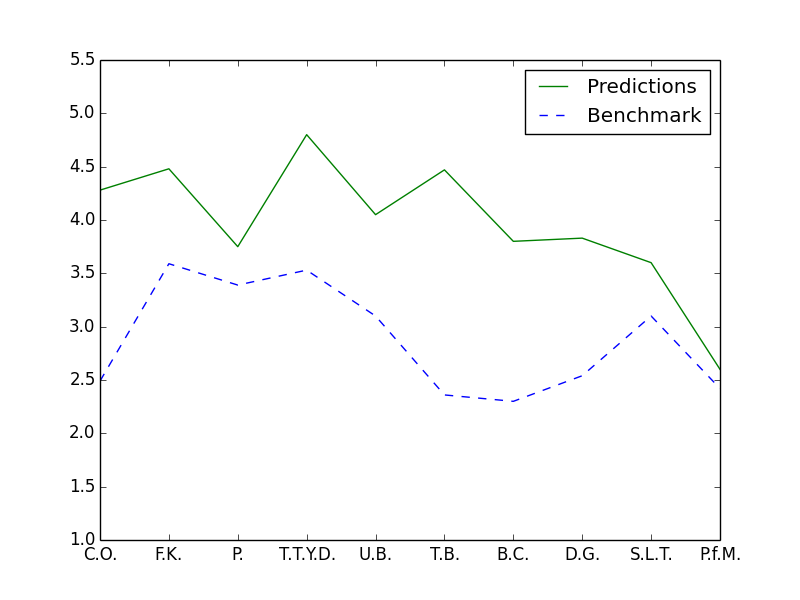
\includegraphics[width=.8\textwidth]{Figures/plots/predictions_benchmark_rand}
  \caption{Run A: Line plot of predictions vs. benchmark value.}
  \label{fig:predictions_benchmark_rand}
\end{figure}

\subsubsection{Noisy Twitter search results}

Most of the Twitter results listed in table~\ref{tab:test_run_all} were in fact not about the movie in question. In fact, \emph{all} the search results that were evaluated on behalf of the first movie, ``Chill Out'', were about watching other movies, and only mention ``chill out'' in the same message more or less at random.

The same is the case for several other movies in the listed sample run.

\subsection{Run B: Sample drawn from IMDB's top 250 list}

This run gives a MAE of 0.38, and a correlational coefficient of 0.40. Again, details are available, in table~\ref{tab:test_run_popular}.

Subsequent runs with the same parameters yield the following:

\begin{enumerate}
  \item MAE: 0.78, correlational coefficient: 0.16
  \item MAE: 0.58, correlational coefficient: -0.27
  \item MAE: 0.52, correlational coefficient: 0.23
\end{enumerate}

The comparative plot in figure~\ref{fig:predictions_benchmark_pop} is better adjusted with regard to overshooting the benchmark values. However, the plot fails to emphasize is that the degree of correlation is approximately the same in both runs.

\begin{figure}[h]
  \centering
    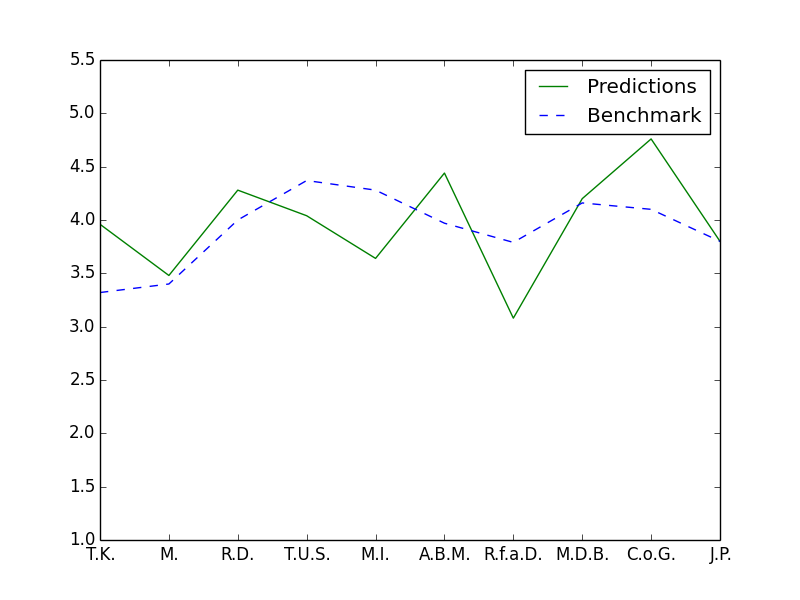
\includegraphics[width=.8\textwidth]{Figures/plots/predictions_benchmark_pop}
  \caption{Run B: Line plot of predictions vs. benchmark value.}
  \label{fig:predictions_benchmark_pop}
\end{figure}

\subsection{Evaluation result comparison} % (fold)
\label{sub:evaluation_result_comparison}

Up to this point, the predictions have only been compared with the benchmarks. Here, they will be compared among themselves.

First, the benchmarks. Let the set of benchmark ratings for run A be denoted $R_A$, and similarly the benchmark ratings from run B $R_B$. As expected, the average benchmark ratings from run B -- the top movies -- are clearly above the ones from run A.

\begin{align}
  \bar{R}_A = 2.882 \\
  \bar{R}_B = 3.919
\end{align}

A difference of more than $1.0$. A number along these lines is what we want to see as the difference between the average predictions from the two runs.

However, when we perform the same mean value comparison for the \emph{predictions} from the two runs, denoted $P_A$ and $P_B$, we see a different pattern:

\begin{align}
  \bar{P}_A = 3.966 \\
  \bar{P}_B = 3.968
\end{align}

A difference of only 0.002 -- a mere nothing.

The difference becomes especially revealing when compared visually, as in figure~\ref{fig:pr_run_comparison}.

This result repeats in approximately the same way for every run: the average rating predictions seem to be completely disassociated with the benchmark ratings of the test set.

\begin{figure}[h]
  \centering
    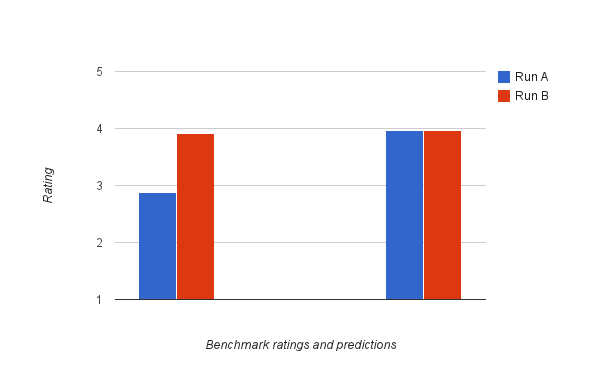
\includegraphics[width=.8\textwidth]{Figures/plots/pr_run_comparison}
  \caption{Comparison of ratings and predictions, per run. Left: ratings, right: predictions.}
  \label{fig:pr_run_comparison}
\end{figure}

% subsection evaluation_run_summary (end)
